\section*{The Workflow}
\label{sec.framework}


Figure~\ref{fig:flow_chart} introduces the proposed workflow.
It can be broken down into five
macro-processes (A)-(E). Compared to
WGCNA, the workflow adds the macro-step (D) and generalizes macro-steps (A)-(C).
\vspace{0.5cm}

% figure 1
\begin{figure}[htbp]
  \centering
    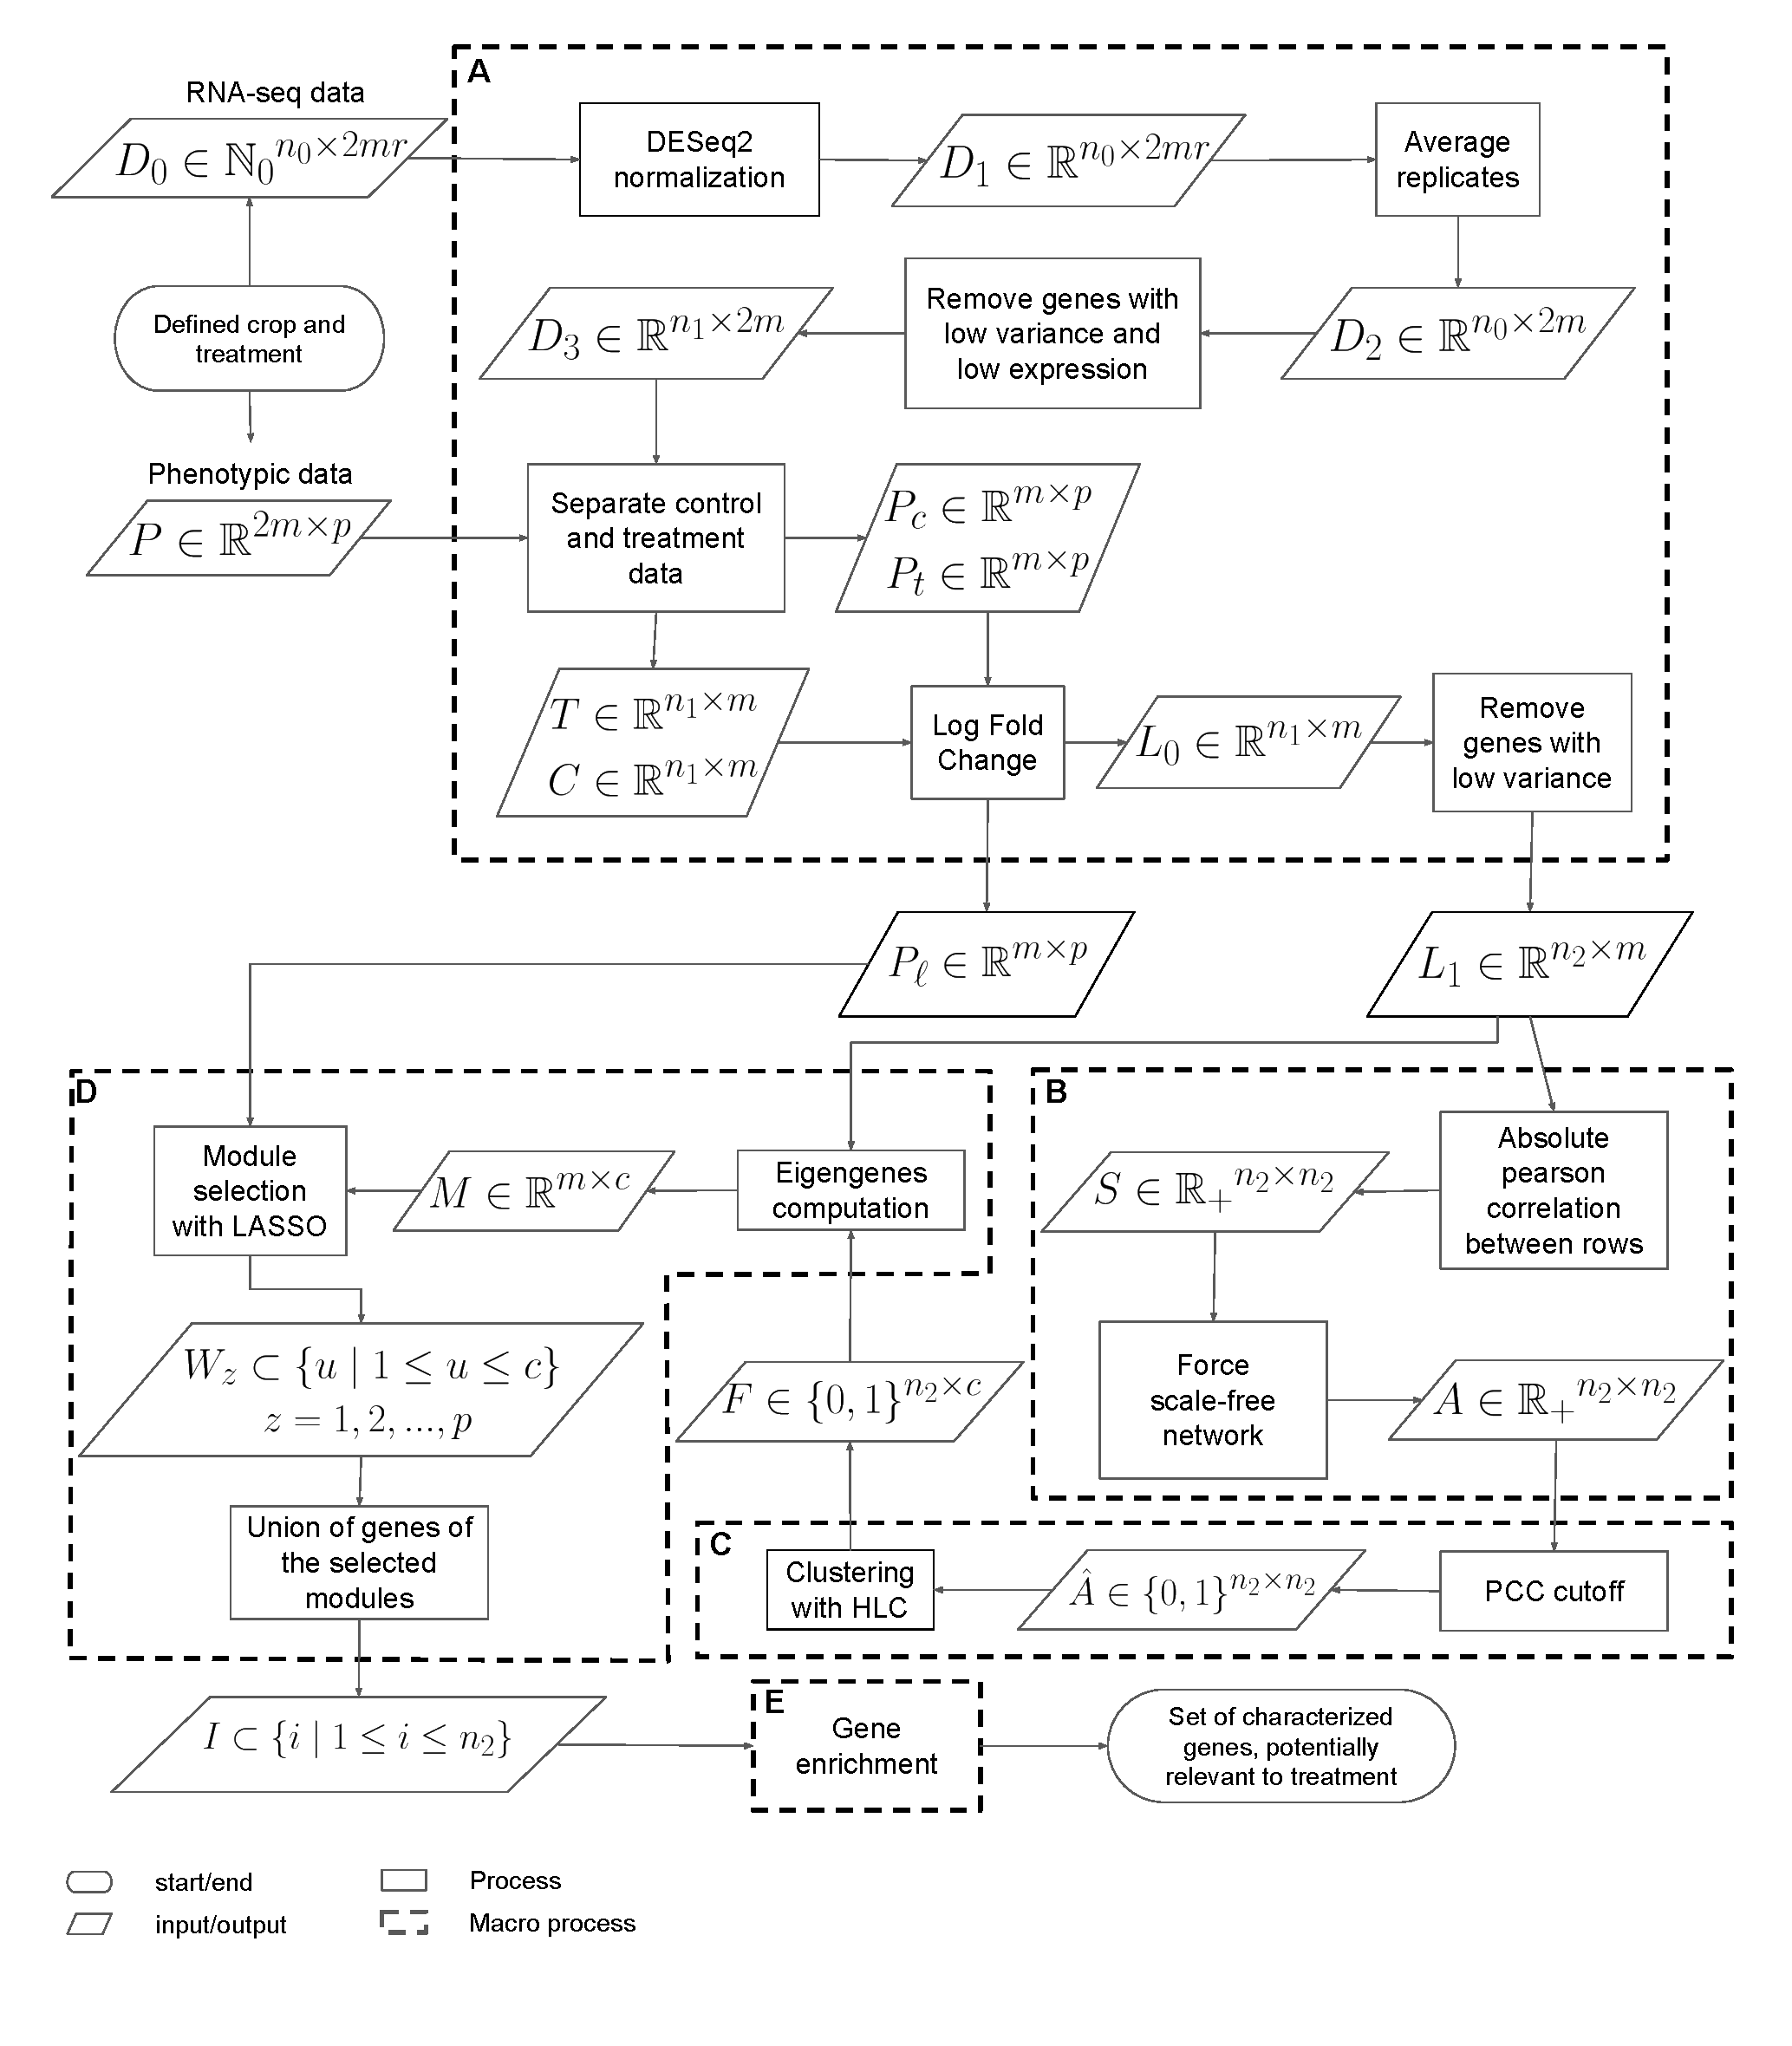
\includegraphics[clip,width=0.96\textwidth]{figures/figure1.pdf}
  \caption[The proposed workflow is broken down into five macro-steps]%
  {The proposed workflow is broken down into five macro-steps:
    A.~Data pre-processing, B.~Co-expression network
    contruction, C.~Identification of co-expression modules,
    D.~Detection of modules association to phenotypic traits, and
    E.~Gene enrichment.}
  \label{fig:flow_chart}
\end{figure}

The input of the workflow includes RNA-seq read counts, representing gene expression
levels. More precisely, the workflow uses $n_0$ gene expression
profiles, measured for $m$ different genotypes 
of $r$ biological replicates (under
control and treatment conditions). This
data is represented as matrix $D_0 \in {\mathbb{N}_0}^{n_0
  \times 2mr}$. To discover key genes and their interaction
with phenotypes related to treatment, the approach also
requires a set of $p$ phenotypic traits, measured for $m$
genotypes. The phenotypic data is captured by matrix $P \in
\mathbb{R}^{2m \times p}$ which contains two phenotypic values per
genotype (under control and treatment
conditions).

\subsection*{A. Data Pre-processing}

The goal of the data pre-processing stage is to build matrices
$P_\ell$ and $L_1$ which represent, respectively, the changes in
phenotypic values and expression levels between control and treatment
condition. In other words, $P_\ell$ and $L_1$ are constructed from RNA-seq and phenotypic data found in matrices $D_0$
and $P$.
\vspace{0.5cm}

A normalization process is applied to interpret RNA-seq data and handle possible
biases affecting the quantification of results. Here,  DESeq2~\cite{love2014moderated}
is used to correct for library size and RNA
composition bias. The normalized
data is represented as a matrix $D_1 \in \mathbb{R}^{n_0 \times 2mr}$,
and the biological replicates of each genotype are averaged and
represented as a matrix $D_2 \in \mathbb{R}^{n_0 \times 2m}$. The
genes exhibiting low variance or low expression are removed from
$D_2$. Consequently, this stage of the approach reduces
the set of genes from a pool of size $n_0$ to $n_1$.
The control and treatment data is separated into the
matrices $C\in \mathbb{R}^{n_1 \times m}$ and $T\in \mathbb{R}^{n_1
  \times m}$, respectively. The matrix entries $c_{ij}$ in $C$ and
$t_{ij}$ in $T$ represent the normalized expression
level of gene $i$ in accession $j$ under control and treatment 
condition, respectively.
Control and treatment data is also separated from
phenotypic data $P$, obtaining the $P_c$ and $P_t$ matrices of
dimensions $m \times p$.
\vspace{0.5cm}

In the above configuration, the changes in expression levels and
phenotypic values between control and treatment conditions are
measured in terms of logarithmic ratios. In the case of expression
levels, the log ratios are represented in the Log Fold Change matrix
$L_0 \in \mathbb{R}^{n_1 \times m}$, where $\ell_{ij}=\log_2
(t_{ij}/c_{ij})$. Similarly, the log ratios of the phenotypic data are
computed and represented in the $P_\ell \in \mathbb{R}^{m \times p}$
matrix.
\vspace{0.5cm}

The final stage of pre-processing is to filter $L_0$ by
removing rows (e.g., genes) with low variance in the differential
expression patterns, obtaining a new matrix $L_1$ of dimensions $n_2
\times m$, with $n_2 \leq n_1$.

\subsection*{B. Construction of the Co-expression Network}

A gene co-expression network connects genes with similar expression
patterns across biological conditions. The purpose of this step is to
describe how to build the co-expression network $A$ from the Log Fold
Change matrix $L_1$, capturing the relationship between genes
according to the change in expression levels between the two studied
conditions. These co-expression patterns are meaningful for the
identification of genes that are not yet associated to treatment response.
\vspace{0.5cm}

The Log Fold Change matrix $L_1$ is used to build the co-expression
network following the first two steps of WGCNA~\cite{langfelder2008wgcna}.
First, the level of
concordance between gene differential expression profiles across
samples is measured. To this end, the absolute value of the Pearson
correlation coefficient is used as the similarity measure between
genes and the resulting values are stored in the similarity matrix
$S\in \mathbb{R_{+}}^{n_2 \times n_2}$. Second, the matrix $S$ is
transformed into an adjacency matrix $A \in \mathbb{R_+}^{n_2\times
  n_2}$ where each entry $a_{ij} = (s_{ij})^\beta $ encodes the
connection strength between each pair of genes. In other words, the
elements of the adjacency matrix are the similarity values up to the
power $\beta > 1$ so that the degree distribution will fit a
scale-free network. These networks contain many nodes with very few
connections and a small number of hubs with high connections. In a
strict scale-free network, the logarithm of $P(k)$ (i.e., the
probability of a node having degree $k$) is approximately inversely
proportional to the logarithm of $k$ (i.e., the degree of a node).
The parameter $\beta$ is chosen to be the smallest value for which the
$R^2$ of the linear regression between $log_{10}(p(k))$ and
$log_{10}(k)$ is closest to $1$ (Here, $R^2 > 0.8$).

\subsection*{C. Identification of Co-expression Modules}

The next step in the workflow is to identifying modules of overlapping communities
from the co-expression network
represented by $A$.  The idea is to cluster genes with similar
patterns of differential expression change. Membership in these
modules may overlap in biological contexts, because modules may be
related to specific molecular, cellular, or tissue functions, and the
biological components (i.e., genes) may be involved in multiple
functions. Unlike WGCNA, the workflow applies 
the Hierarchical Link Clustering (HLC) algorithm (overviewed in the 
\hyperref[sec.prelim]{Preliminaries} section) to
detect overlapping rather than non-overlapping communities.
%Section~\ref{sec.prelim}).
\vspace{0.5cm}

First, the adjacency matrix $A$ is transformed into an unweighted
network $\hat{A} \in \{0,1\}^{n_2 \times n_2}$.
To this end, the Pearson Correlation Coefficient
(PCC) cutoff is determined using the approach described
in~\cite{aoki2007approaches}. The number of nodes, edges, and the
network density is determined for different PCC cutoffs. 
In a neighborhood of the optimal PCC cutoff
the number of nodes presents a linear
decrease and the density of the network reaches its minimum, while
below this value the number of edges rapidly increases. Following this
observation, a cutoff is selected such that gene pairs which have a
correlation score higher than the threshold are considered to have
a significant level of co-expression. Above the cutoff, the entries of
matrix $A$ become $1$ and below the cutoff $A$ values become $0$. The
HLC algorithm organizes the $n_2$ genes of matrix $\hat{A}$ into $c$~modules, where each gene can belong to zero or multiple modules.
This information is represented as an affiliation matrix $F \in
\{0,1\}^{n_2 \times c}$, where $f_{iu} = 1$ if node $i$ is a member of
module $u$ (and $f_{iu}=0$ otherwise).

\subsection*{D. Detection of Modules Association to Phenotypic Traits}

To identify the most relevant modules, associated
with the phenotypic response to a specific treatment,
the proposed workflow uses LASSO. Specifically, each module is
represented by an eigengene, which is defined as the first principal
component of such module. An eigengene can be seen as an average
differential expression profile for each community: it is computed
from the Log Fold Change Matrix $L_1$ and the affiliation matrix
$F$. Given a module $u$, the affiliation matrix $F$ is used to identify
the genes belonging to $u$ and then the corresponding rows of the
matrix $L_1$ are selected to compute the first principal component of
$u$. Each principal component becomes a column of the matrix $M \in
\mathbb{R}^{m \times c}$.  These profiles are associated with each
phenotypic trait using
LASSO.  In this context, the eigengenes (i.e., the columns
of $M$) act as regressor variables and each phenotypic trait (i.e.,
each column of $P_\ell$) is used as an outcome variable.
\vspace{0.5cm}

The output after applying LASSO is a set $W_z$ of modules for each
phenotypic trait $z$, where $W_z \subset \{u \mid 1 \leq u \leq c\}$
for $z= 1,2,..,p$. The target genes $I$ for downstream analysis
are the union of genes
belonging to the selected modules; that is $I = \cup_{z=1}^{p} W_z$,
where $I \subset \{i \mid 1 \leq i \leq n_2\}$.

\subsection*{E. Gene Enrichment}

The goal of this final step of the process is to annotate with
additional information the genes identified in previous stages,
helping to elucidate their possible behavior and role in the response
to the studied treatment.
\vspace{0.5cm}

A crucial step is to identify the differentially expressed genes in
set $I$. That is, to select the genes in $I$ that have an absolute
value of the Log Fold Change of at least $2$ ($|\ell_{ij}|\geq 2$) for
at least one sample. This represents genes whose expression level is
quadrupled (up or down) from the control to treatment condition; they are
target genes.
\vspace{0.5cm}

Furthermore, functional category enrichment can be carried out by, e.g., searching
for gene ontology annotations in databases such as
QuickGO~\cite{binns2009quickgo}. Such annotations can provide evidence
of biological implications of the target genes in the
treatment-tolerance mechanisms. Furthermore, QuickGO can be used to
identify the protein products of genes, which can be used to
perform additional analysis that provides new insights into how target genes are
involved in functional pathways that can be related to treatment.
Such analysis includes a review of reported
protein-protein interactions in databases such as
STRING~\cite{szklarczyk2016string}. The protein interactions include direct
(physical) and indirect (functional) associations. They stem from
computational prediction, knowledge transfer between organisms, and
interactions aggregated from other (primary) databases. The search for unknown interactions would extend the workflow with additional steps.
